\documentclass[8pt, compress]{beamer}
\usepackage[utf8]{inputenc}
\usepackage{graphicx}
\usepackage{amsmath}
\usepackage{amssymb}
\usepackage{tikz}
\usetikzlibrary{positioning}

\usetheme{CambridgeUS}
\usecolortheme{beaver}

\setbeamertemplate{footline}
{
  \hbox{\begin{beamercolorbox}[wd=1\paperwidth,ht=2.25ex,dp=1ex,right]{framenumber}%
      \usebeamerfont{framenumber}\insertframenumber{} / \inserttotalframenumber\hspace*{2ex}
    \end{beamercolorbox}}%
  \vskip0pt%
}
\useoutertheme{miniframes}

%%% For XOR Symbol
\tikzset{XOR/.style={draw,circle,append after command={
        [shorten >=\pgflinewidth, shorten <=\pgflinewidth,]
        (\tikzlastnode.north) edge (\tikzlastnode.south)
        (\tikzlastnode.east) edge (\tikzlastnode.west)
        }
    }
}
%%% For changing color
\usetikzlibrary{overlay-beamer-styles}

\title{Polar Codes}
\author{Aayush Rajesh, Ronil Mandavia}
\institute{Department of Electrical Engineering \\ IIT Bombay}
\date{}

\begin{document}

\frame{\titlepage}

\begin{frame}{Outline}
    \tableofcontents
\end{frame}

\section{Introduction}

\begin{frame}{Overview}
\begin{itemize}
    \item<1-> Polar Codes were introduced by Erdal Arıkan in \cite{5075875}, and are constructed by exploiting a phenomenon known as \textbf{channel polarization}.
    \item<2-> It can be shown that these codes achieve Shannon's Capacity.
    \item<3-> We shall look to motivate the polarization phenomenon to understand how these codes achieve capacity. Efficient encoding and decoding procedures shall also be covered.
\end{itemize}
\end{frame}

\begin{frame}
\frametitle{Information Theoretic Measures}
\begin{itemize}
    
\item<1-> \textbf{Entropy:} Entropy measures the average uncertainty in a random variable.

$$
H(X) = - \sum_{x \in \mathcal{X}} p(x) \log p(x)
$$ 

\onslide<2->{
$$
H(Y|X) = - \sum_{x \in \mathcal{X}} \sum_{y \in \mathcal{Y}} p(x, y) \log p(y|x)
$$
}

\item<3-> \textbf{Mutual Information:} The reduction in uncertainty in one random variable due to knowledge of another.

$$
I(X; Y) = H(X) - H(X|Y) \onslide<4->{ = H(Y) - H(Y|X)}
$$

\item<5-> \textbf{Chain Rule:} $$I(X, Y; Z) = I(X; Z) + I(Y; Z|X)$$

\end{itemize}

\end{frame}

\begin{frame}{The Channel}
\onslide<1->{
\begin{center}
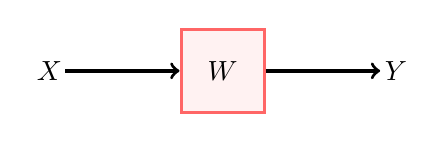
\begin{tikzpicture}[channel/.style={rectangle, draw=red!60, fill=red!5, very thick, minimum size=30}]
    \node[channel](channel){$W$};
    \node[] at (-2.2,0) {$X$};
    \node[] at (2.2,0) {$Y$};
    \draw[->, very thick] (-2,0) to (channel.west); 
    \draw[->, very thick] (channel.east) to (2, 0);
\end{tikzpicture}
\end{center}
}

\begin{itemize}
    \item<1-> Channel $W : \mathcal{X} \to \mathcal{Y}$, characterized by \textbf{transition probabilities} $W(y|x)$.
    \item<2-> The maximum rate of reliable communication over this B-DMC\footnote<2->{Binary-Discrete Memoryless Channel} is the \textbf{capacity} and is given by
    $$
    C = \max_{p(x)} I(X; Y)
    $$
    \item<3-> There are two classes for which analysis of communication is trivial
    \begin{itemize}
        \item<3-> Perfect Channels: $C = 1$
        \item<3-> Useless Channels: $C = 0$
    \end{itemize}
\end{itemize}

\end{frame}

\begin{frame}{Channel Capacity}
\onslide<1->{A simple analysis of channel capacity can be undertaken for the BEC(p) channel. We have $W(0|0) = W(1|1) = 1-p$ and $W(\textcolor{red}{?}|0) =W(\textcolor{red}{?}|1) = p$. The mutual information of the channel can be evaluated as}

\begin{equation*}
\begin{split}
\onslide<2->{I(X;Y) &= H(X) - H(X|Y)\\}
\onslide<3->{ &= H(X) - p_Y(\textcolor{red}{?})H(X|\textcolor{red}{?}) - p_Y(0)H(X|0) - p_Y(1)H(X|1)\\}
\uncover<4->{ \alt<5->{&= (1-p)H(X)}{&= H(X) - pH(X) - 0 - 0}}
\end{split}
\end{equation*}

\onslide<6->{This quantity is maximized when $X \sim \text{Ber}\left(\frac{1}{2}\right)$, giving us $C = 1 - p$ for a BEC(p) channel. Through a similar analysis, we can obtain that $C = 1 - H(p)$ for a BSC(p) channel.}
\end{frame}

\section{Polarization}

\begin{frame}{Combining Channels}

\begin{columns}
    \begin{column}{0.6\linewidth}
        \begin{itemize}
            \item<1-> We can denote $X_1 = U_1 \oplus U_2$ and $X_2 = U_2$. There is an invertible transformation between $(U_1, U_2)$ and ($X_1, X_2)$.
            \item<2-> The capacity of this joint ensemble is
            \begin{equation*}
            \begin{split}
            2C(W) &= I(X_1 X_2; Y_1 Y_2) = I(U_1 U_2; Y_1 Y_2)\\
            \onslide<3->{ &= I(U_1; Y_1 Y_2) + I(U_2; Y_1 Y_2 | U_1)\\}
            \onslide<4->{ &= I(U_1; Y_1 Y_2) + I(U_2; Y_1 Y_2 U_1)\\}
            \only<5>{ &= C(W^-) + C(W^+)\\}
            \only<6>{ &= C(\textcolor{red}{W^-}) + C(W^+)\\}
            \only<7>{ &= C(W^-) + C(\textcolor{green}{W^+})\\}
            \onslide<8->{ &= C(W^-) + C(W^+)\\}
            \end{split}
            \end{equation*}
        \end{itemize}
    \end{column}
    \begin{column}{0.37\linewidth}
        \begin{tikzpicture}[channel/.style={rectangle, draw=black!80, fill=white!5, very thick, minimum size=30}, scale=0.8, every node/.style={scale=0.8}]
            \node[channel](channel1){$W$};
            \node[channel](channel2) at (0, -1.5) {$W$};
            \alt<7>{\node[] at (-2.5,0) {\textcolor{green}{$U_1$}}}{\node[] at (-2.5,0) {$U_1$}};
            %\alt<7>{\node[] at (-2.5,0) {\textcolor{green}{$U_1$}}}{\node[] at (-2.5,0) {$U_1$}};
            \alt<6>{\node[] at (2,0) {\textcolor{red}{$Y_1$}}}{\alt<7>{\node[] at (2,0) {\textcolor{green}{$Y_1$}}}{\node[] at (2,0) {$Y_1$}}};
            \alt<6>{\node[] at (-2.5,-1.5) {\textcolor{black!40}{$U_2$}}}{\node[] at (-2.5,-1.5) {$U_2$}};
            \alt<6>{\node[] at (2, -1.5) {\textcolor{red}{$Y_2$}}}{\alt<7>{\node[] at (2, -1.5) {\textcolor{green}{$Y_2$}}}{\node[] at (2, -1.5) {$Y_2$}}};
            \node[XOR, thick] at (-1.5, 0) {};
            \node[circle, fill, inner sep = 1.5pt] at (-1.5, -1.5) {};
            \draw[->, thick] (-2.3,0) to (-1.7, 0); 
            \draw[->, thick] (-1.3,0) to (channel1.west); 
            \draw[->, thick] (channel1.east) to (1.8, 0);
            \draw[->, thick] (-2.3,-1.5) to (channel2.west); 
            \draw[->, thick] (channel2.east) to (1.8, -1.5);
            \draw[->, thick] (-1.5,-1.5) to (-1.5, -0.2); 
        \end{tikzpicture}
    \end{column}
\end{columns}

\begin{itemize}
    \item<8-> We now have two different ``channels'', $W^-$ and $W^+$. Total channel capacity is conserved, but distributed unevenly. One is better than the original channel, and the other worse. This is at the heart of polarization.
\end{itemize}

\end{frame}

\begin{frame}{New Channel Capacities: BEC Case}
    \begin{columns}
        \begin{column}{0.45\linewidth}
            \begin{itemize}
                \item<1-> Channel $W^-$ has input $U_1$ and output
                \begin{flushleft}
                $$
                (Y_1, Y_2) = 
                \begin{cases}
                (X_1, X_2) &\text{w.p. }(1-p)^2 \\
                (\textcolor{red}{? }, X_2) &\text{w.p. }p(1-p) \\
                (X_1, \textcolor{red}{?}) &\text{w.p. }(1-p)p \\
                (\textcolor{red}{? }, \textcolor{red}{?}) &\text{w.p. }p^2 \\
                \end{cases}
                $$
                \end{flushleft}
                \item<2-> First case is good, other three can be treated as erasure. Therefore $W^-$ is BEC($p^-$), where $p^- = 2p-p^2$.\\
                
            \end{itemize}
        \end{column}
        \begin{column}{0.55\linewidth}
            \begin{itemize}
                \item<3-> Channel $W^+$ has input $U_2$ and output
                \begin{flushleft}
                $$
                (Y_1, Y_2, U_1) = 
                \begin{cases}
                (X_1, X_2, U_1) &\text{w.p. }(1-p)^2 \\
                (\textcolor{red}{? }, X_2, U_1) &\text{w.p. }p(1-p) \\
                (X_1, \textcolor{red}{?}, U_1) &\text{w.p. }(1-p)p \\
                (\textcolor{red}{? }, \textcolor{red}{?}, U_1) &\text{w.p. }p^2 \\
                \end{cases}
                $$
                \end{flushleft}
                \item<4-> Last case can be treated as erasure, other three are good. Therefore $W^+$ is BEC($p^+$), where $p^+ = p^2$.\\
                
            \end{itemize}
        \end{column}
    \end{columns}
    \vspace{6pt}
    \begin{flushleft}
        \onslide<5->{ Note that $p^- \geq p^+$ for all $p \in [0, 1]$. Therefore, we have the relation \footnote<5->{In general, $C(W^+) = 2C(W) - C^2(W)$ and $C(W^-) = C^2(W)$. Refer to \cite{5075875} for details.} 
        $$
        C(W^-) \leq C(W) \leq C(W^+)
        $$}
    \end{flushleft}
    
    
\end{frame}

\appendix
\section*{References}
\begin{frame}{References}
\bibliographystyle{ieeetr}
  \bibliography{references}
\end{frame}

\end{document}
